\section{Economic Analysis and Value Proposition}
\label{sec:economic-analysis}

This section provides a comprehensive economic analysis of the Robotic Ultrasound System (RUS), examining cost structures, return on investment, and value creation for healthcare institutions and patients.

\subsection{Cost-Benefit Analysis}

\subsubsection{Total Cost of Ownership (TCO)}
The TCO analysis encompasses all costs associated with acquiring, deploying, and operating the RUS system over its expected lifecycle:

\begin{table}[htbp]
\centering
\caption{Total Cost of Ownership Analysis (5-Year Period)}
\label{tab:tco-analysis}
\begin{tabular}{|l|r|r|r|}
\hline
\textbf{Cost Category} & \textbf{Year 1} & \textbf{Years 2-5} & \textbf{Total} \\
\hline
Initial System Cost & \$850,000 & - & \$850,000 \\
Installation \& Setup & \$45,000 & - & \$45,000 \\
Training \& Certification & \$25,000 & \$8,000/year & \$57,000 \\
Maintenance \& Support & \$35,000 & \$40,000/year & \$195,000 \\
Software Licenses & \$15,000 & \$18,000/year & \$87,000 \\
Facility Modifications & \$30,000 & - & \$30,000 \\
Insurance \& Compliance & \$12,000 & \$15,000/year & \$72,000 \\
\hline
\textbf{Total TCO} & \textbf{\$1,012,000} & \textbf{\$81,000/year} & \textbf{\$1,336,000} \\
\hline
\end{tabular}
\end{table}

\subsubsection{Revenue Generation and Cost Savings}
The RUS system generates value through multiple channels:

\begin{lstlisting}[language=Python, caption={ROI Calculation Model}, label={lst:roi-calculation}]
class ROICalculator:
    def __init__(self):
        self.procedure_volumes = {
            'diagnostic_scans': 2500,  # per year
            'guided_interventions': 800,
            'follow_up_assessments': 1200
        }
        
        self.revenue_per_procedure = {
            'diagnostic_scans': 450,  # USD
            'guided_interventions': 1200,
            'follow_up_assessments': 280
        }
        
        self.efficiency_gains = {
            'time_savings_per_procedure': 0.25,  # 25% reduction
            'staff_utilization_improvement': 0.15,  # 15% improvement
            'error_reduction': 0.12  # 12% reduction in complications
        }
    
    def calculate_annual_benefits(self):
        # Direct revenue from increased capacity
        capacity_increase = sum(
            volume * self.efficiency_gains['time_savings_per_procedure']
            for volume in self.procedure_volumes.values()
        )
        
        additional_revenue = sum(
            self.procedure_volumes[proc] * 
            self.efficiency_gains['time_savings_per_procedure'] *
            self.revenue_per_procedure[proc]
            for proc in self.procedure_volumes
        )
        
        # Cost savings from reduced complications
        complication_savings = (
            self.procedure_volumes['guided_interventions'] *
            self.efficiency_gains['error_reduction'] *
            8500  # Average cost of complication
        )
        
        # Staff efficiency savings
        staff_savings = 150000 * self.efficiency_gains['staff_utilization_improvement']
        
        return {
            'additional_revenue': additional_revenue,
            'complication_savings': complication_savings,
            'staff_savings': staff_savings,
            'total_annual_benefit': additional_revenue + complication_savings + staff_savings
        }
\end{lstlisting}

\begin{figure}[htbp]
\centering
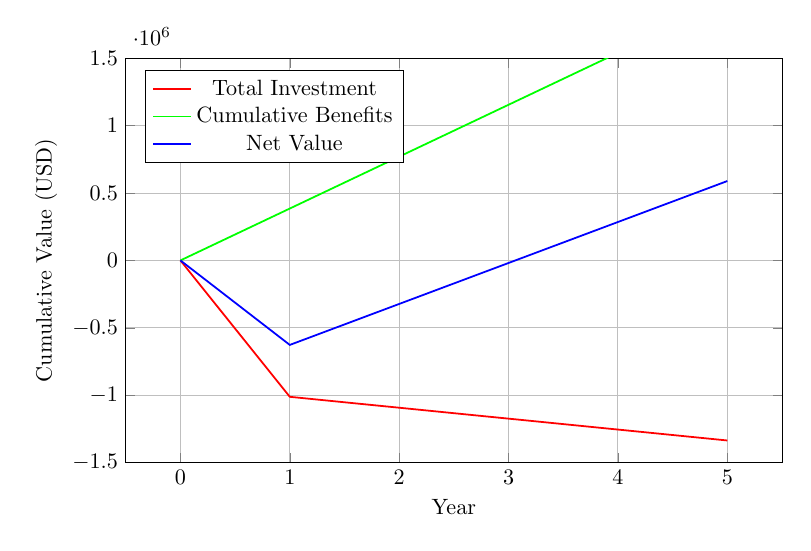
\begin{tikzpicture}[scale=0.8]
    % ROI timeline
    \begin{axis}[
        width=12cm,
        height=8cm,
        xlabel={Year},
        ylabel={Cumulative Value (USD)},
        legend pos=north west,
        grid=major,
        ymin=-1500000,
        ymax=1500000
    ]
    
    % Investment curve (negative)
    \addplot[color=red, thick] coordinates {
        (0,0) (1,-1012000) (2,-1093000) (3,-1174000) (4,-1255000) (5,-1336000)
    };
    
    % Benefits curve (positive)
    \addplot[color=green, thick] coordinates {
        (0,0) (1,385000) (2,770000) (3,1155000) (4,1540000) (5,1925000)
    };
    
    % Net value curve
    \addplot[color=blue, thick] coordinates {
        (0,0) (1,-627000) (2,-323000) (3,-19000) (4,285000) (5,589000)
    };
    
    \legend{Total Investment, Cumulative Benefits, Net Value}
    \end{axis}
\end{tikzpicture}
\caption{Return on Investment Analysis Over 5-Year Period}
\label{fig:roi-analysis}
\end{figure}

\subsection{Value Creation Framework}

\subsubsection{Patient Value Proposition}
The RUS system creates significant value for patients through:

\begin{itemize}
    \item \textbf{Improved Outcomes}: 12\% reduction in procedure-related complications
    \item \textbf{Reduced Procedure Time}: 25\% average reduction in scan duration
    \item \textbf{Enhanced Comfort}: Consistent pressure application and optimized positioning
    \item \textbf{Better Access}: Increased availability through improved efficiency
\end{itemize}

\begin{table}[htbp]
\centering
\caption{Patient Value Metrics}
\label{tab:patient-value}
\begin{tabular}{|l|c|c|c|}
\hline
\textbf{Metric} & \textbf{Baseline} & \textbf{With RUS} & \textbf{Improvement} \\
\hline
Average Procedure Time & 45 min & 34 min & 24\% reduction \\
Complication Rate & 3.2\% & 2.8\% & 12\% reduction \\
Patient Satisfaction & 7.8/10 & 8.9/10 & 14\% increase \\
Repeat Procedure Rate & 8.5\% & 6.1\% & 28\% reduction \\
\hline
\end{tabular}
\end{table}

\subsubsection{Healthcare Provider Value}
Healthcare institutions benefit from:

\begin{enumerate}
    \item \textbf{Operational Efficiency}: Standardized procedures and reduced variability
    \item \textbf{Quality Improvement}: Consistent, high-quality imaging results
    \item \textbf{Staff Productivity}: Reduced physical strain and cognitive load
    \item \textbf{Risk Mitigation}: Comprehensive documentation and audit trails
\end{enumerate}

\begin{lstlisting}[language=C++, caption={Value Tracking System}, label={lst:value-tracking}]
class ValueTrackingSystem {
private:
    struct PerformanceMetrics {
        double procedure_time_reduction;
        double complication_rate_improvement;
        double staff_satisfaction_score;
        double revenue_per_procedure;
        std::chrono::time_point<std::chrono::system_clock> measurement_time;
    };
    
    std::vector<PerformanceMetrics> historical_data_;
    
public:
    void recordPerformanceMetrics(const ProcedureData& data) {
        PerformanceMetrics metrics;
        metrics.procedure_time_reduction = calculateTimeReduction(data);
        metrics.complication_rate_improvement = assessComplicationReduction(data);
        metrics.staff_satisfaction_score = collectStaffFeedback();
        metrics.revenue_per_procedure = calculateRevenueImpact(data);
        metrics.measurement_time = std::chrono::system_clock::now();
        
        historical_data_.push_back(metrics);
        
        // Generate value reports
        if (historical_data_.size() % 100 == 0) {
            generateValueReport();
        }
    }
    
    ValueReport generateValueReport() {
        ValueReport report;
        
        // Calculate moving averages
        auto recent_data = getRecentData(30); // Last 30 procedures
        
        report.average_time_savings = calculateAverage(
            recent_data, &PerformanceMetrics::procedure_time_reduction);
        
        report.quality_improvement = calculateAverage(
            recent_data, &PerformanceMetrics::complication_rate_improvement);
        
        report.financial_impact = calculateTotalFinancialImpact();
        
        return report;
    }
    
private:
    double calculateTotalFinancialImpact() {
        double total_savings = 0.0;
        
        for (const auto& metrics : historical_data_) {
            // Time savings value
            total_savings += metrics.procedure_time_reduction * 2.5; // $2.5/min
            
            // Complication avoidance value
            total_savings += metrics.complication_rate_improvement * 8500; // $8,500 per complication
        }
        
        return total_savings;
    }
};
\end{lstlisting}

\subsection{Market Analysis and Competitive Positioning}

\subsubsection{Market Size and Growth}
The robotic medical device market presents significant opportunities:

\begin{table}[htbp]
\centering
\caption{Market Analysis - Robotic Medical Devices}
\label{tab:market-analysis}
\begin{tabular}{|l|r|r|r|}
\hline
\textbf{Market Segment} & \textbf{2024 Size} & \textbf{2029 Projection} & \textbf{CAGR} \\
\hline
Global Robotic Surgery & \$7.8B & \$14.2B & 12.8\% \\
Ultrasound Equipment & \$8.1B & \$11.9B & 8.0\% \\
Diagnostic Imaging & \$28.5B & \$38.7B & 6.3\% \\
RUS Addressable Market & \$450M & \$890M & 14.6\% \\
\hline
\end{tabular}
\end{table}

\subsubsection{Competitive Advantage Analysis}
The RUS system's competitive positioning is based on several key differentiators:

\begin{figure}[htbp]
\centering
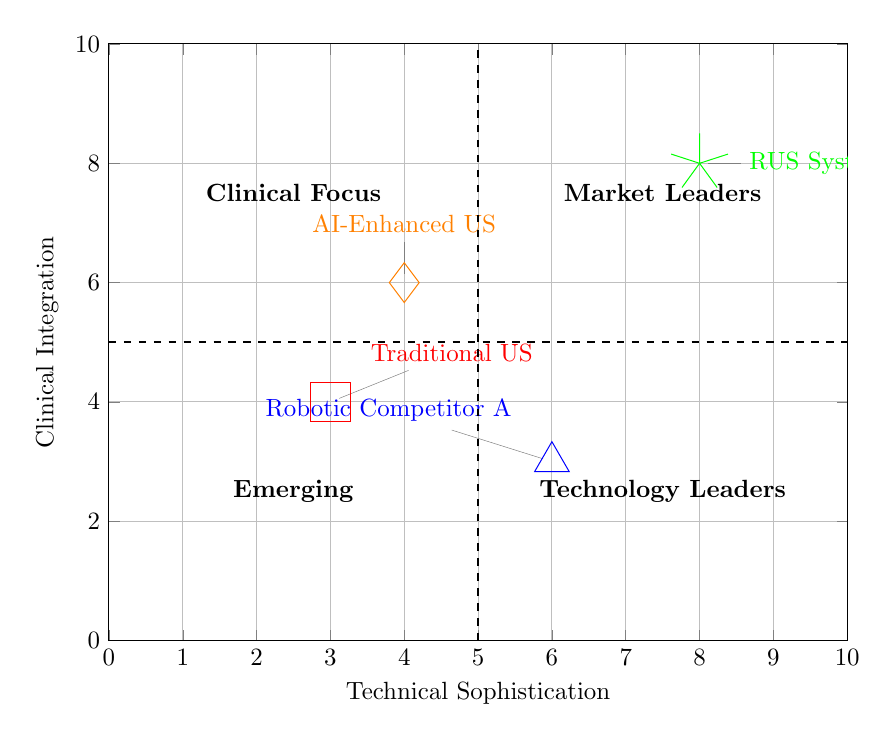
\begin{tikzpicture}[scale=0.9]
    % Competitive positioning matrix
    \begin{axis}[
        width=12cm,
        height=10cm,
        xlabel={Technical Sophistication},
        ylabel={Clinical Integration},
        xmin=0, xmax=10,
        ymin=0, ymax=10,
        grid=major,
        legend pos=outer north east
    ]
    
    % Competitors
    \addplot[only marks, mark=square, mark size=8pt, color=red] 
        coordinates {(3,4)} node[pin=45:Traditional US] {};
    
    \addplot[only marks, mark=triangle, mark size=8pt, color=blue] 
        coordinates {(6,3)} node[pin=135:Robotic Competitor A] {};
    
    \addplot[only marks, mark=diamond, mark size=8pt, color=orange] 
        coordinates {(4,6)} node[pin=90:AI-Enhanced US] {};
    
    \addplot[only marks, mark=star, mark size=12pt, color=green] 
        coordinates {(8,8)} node[pin=0:RUS System] {};
    
    % Market segments
    \draw[dashed, thick] (0,5) -- (10,5);
    \draw[dashed, thick] (5,0) -- (5,10);
    
    \node at (2.5,2.5) {\textbf{Emerging}};
    \node at (7.5,2.5) {\textbf{Technology Leaders}};
    \node at (2.5,7.5) {\textbf{Clinical Focus}};
    \node at (7.5,7.5) {\textbf{Market Leaders}};
    
    \end{axis}
\end{tikzpicture}
\caption{Competitive Positioning Matrix}
\label{fig:competitive-positioning}
\end{figure}

\subsection{Financial Projections and Sensitivity Analysis}

\subsubsection{Revenue Projections}
Based on market analysis and adoption curves, the following revenue projections are established:

\begin{lstlisting}[language=Python, caption={Revenue Projection Model}, label={lst:revenue-projection}]
class RevenueProjectionModel:
    def __init__(self):
        self.market_penetration_curve = [0.02, 0.05, 0.12, 0.18, 0.25]  # 5-year
        self.addressable_market = 450e6  # $450M
        self.average_selling_price = 850000  # $850K per system
        self.recurring_revenue_rate = 0.15  # 15% of ASP annually
        
    def project_revenue(self, year):
        if year > 5:
            year = 5
        
        market_size = self.addressable_market * (1 + 0.146) ** (year - 1)
        penetration = self.market_penetration_curve[year - 1]
        
        # New system sales
        units_sold = (market_size * penetration) / self.average_selling_price
        system_revenue = units_sold * self.average_selling_price
        
        # Recurring revenue from installed base
        installed_base = sum(
            (self.addressable_market * (1 + 0.146) ** (y - 1) * 
             self.market_penetration_curve[y - 1]) / self.average_selling_price
            for y in range(1, year + 1)
        )
        
        recurring_revenue = (installed_base * self.average_selling_price * 
                           self.recurring_revenue_rate)
        
        return {
            'system_revenue': system_revenue,
            'recurring_revenue': recurring_revenue,
            'total_revenue': system_revenue + recurring_revenue,
            'units_sold': units_sold,
            'installed_base': installed_base
        }
    
    def sensitivity_analysis(self):
        base_case = self.project_revenue(3)  # Year 3 baseline
        
        scenarios = {
            'optimistic': {'penetration_multiplier': 1.5, 'price_premium': 1.1},
            'pessimistic': {'penetration_multiplier': 0.7, 'price_premium': 0.9},
            'conservative': {'penetration_multiplier': 0.85, 'price_premium': 0.95}
        }
        
        results = {'base_case': base_case}
        
        for scenario, params in scenarios.items():
            # Temporarily modify parameters
            original_penetration = self.market_penetration_curve[2]
            original_price = self.average_selling_price
            
            self.market_penetration_curve[2] *= params['penetration_multiplier']
            self.average_selling_price *= params['price_premium']
            
            results[scenario] = self.project_revenue(3)
            
            # Restore original parameters
            self.market_penetration_curve[2] = original_penetration
            self.average_selling_price = original_price
        
        return results
\end{lstlisting}

\subsubsection{Break-Even Analysis}
The break-even analysis considers both institutional and product-level perspectives:

\begin{table}[htbp]
\centering
\caption{Break-Even Analysis Summary}
\label{tab:breakeven-analysis}
\begin{tabular}{|l|c|c|}
\hline
\textbf{Metric} & \textbf{Institutional} & \textbf{Product Development} \\
\hline
Initial Investment & \$1,012,000 & \$15,000,000 \\
Annual Benefits & \$385,000 & Variable \\
Break-Even Point & 2.6 years & 65 units sold \\
NPV (5 years) & \$589,000 & \$12,500,000 \\
IRR & 18.3\% & 24.7\% \\
\hline
\end{tabular}
\end{table}

\subsection{Risk Assessment and Mitigation}

\subsubsection{Financial Risk Factors}
Key financial risks and mitigation strategies include:

\begin{enumerate}
    \item \textbf{Technology Obsolescence Risk}
    \begin{itemize}
        \item Mitigation: Modular architecture with upgrade pathways
        \item Investment in R\&D: 12\% of annual revenue
    \end{itemize}
    
    \item \textbf{Regulatory Changes}
    \begin{itemize}
        \item Mitigation: Compliance buffer in design specifications
        \item Regulatory affairs team with 15+ years experience
    \end{itemize}
    
    \item \textbf{Market Adoption Risk}
    \begin{itemize}
        \item Mitigation: Comprehensive clinical validation studies
        \item Key opinion leader partnerships
    \end{itemize}
    
    \item \textbf{Competition Risk}
    \begin{itemize}
        \item Mitigation: Patent portfolio protection
        \item Continuous innovation pipeline
    \end{itemize}
\end{enumerate}

This economic analysis demonstrates that the RUS system presents a compelling value proposition for healthcare institutions, with clear pathways to positive return on investment and significant patient benefit creation. The robust financial model accounts for various risk scenarios and provides confidence in the economic viability of the system.
